\documentclass[a4paper,12pt]{article}
\usepackage{graphicx,url,amsmath}

\begin{document}

% Plan

%     -description of the jacobi solver

%     --mathematical formula

%     -memory layout, code balance flop/byte

%     -main ideas to improve cache utilisation
%       --blocking, time skewed
%       -- what about GPU?
%       --diagram
%       --cite the collected papers 

%    -code presentation
%    --general presentation
%    --command line arguments
%    --run script; data collection

%   -example of data (Ivy Bridge, Phi, GPU)

\section{Introduction}

In this report we present the main features of the Jacobi test code
(JTC) (\url{http://ccpforge.cse.rl.ac.uk/gf/project/asearchtest}), which
measures the performance of several variants of parallel Jacobi
method written in OpenMP and CUDA. Besides
the numerical kernels JTC has a  command line interface and a
timing module. Documentation for the comand line options is provided
in the README file. The timing data is generated in a format suitable
for gnuplot, a bash script is provided for systematic data collection
across a number of platforms.

In JTC the second order Laplacian
discretisation is used to to generate the standard iterative rule
\begin{equation}
u^{(new)}_{i,j,k}=\frac{1}{6}(u^{(old)}_{i-1,j,k}+u^{(old)}_{i+1,j,k}+u^{(old)}_{i,j-1,k}+u^{(old)}_{i,j+1,k}+u^{(old)}_{i,j,k-1}+u^{(old)}_{i,j,k+1})
\ ,
\end{equation} 
on a cuboid $3$D grid with zero boundary condition. 
The iteration sequence starts form an eigenvector of the
Jacobi smoother. This allows for a simple correctness test as the ratio
of $L_2$ norms between two consecutive vectors is the associated eigenvalue
 at every iteration step.  The number of iteration can be controlled by
an input parameter.
 
 JTC has three algorithms written in OpenMP
 and two in CUDA. The OpenMP version contains the standard three
 nested loops, blocked loops and time skewed loops.  CUDA version
 contains standard iteration in $z$ direction with $2$D blocks of
 threads and the same iteration with shared memory enabled to
 store the data in the 2D block. The algorithm and its parameters can
 be selected at the run time with the help of command line arguments.

 The performance of various versions of Jacobi and related iterative
 algorithms for partial differential equations is discussed in detail
 in the recent literature both for multicore CPUs
 \cite{Kamil,Shah,Treibig} and for manycore GPUs \cite{Holewinski}.
 We review briefly the basic ideas used for the performace bound
 estimates for CPU and GPUs and derive some simple expressions which
 should help the reader to gauge the data produced by JTC.  In the
 following we choose as performance metric the number of grid points
 updates per second (LUPS).

\subsection*{ a) CPU}

Multicore CPU use instruction level parallelism, speculative branching,
vectorisation, threading and hierarchies of cache memories
to achieve high performance. 
The Jacobi iteration performance has two limit regimes controlled by the
grid size. For small grids, which fit in in L1 cache, the top speed is
determined by the number of cycles needed to load and store  data
in registers (because the number floating point operations per variable
is small we can assume that floating point computation is overlapped with load
and store operation). For an 8 cores Intel Sandy Bridge processor
which can execute 1/2 store and 1 load vector registers per cycle  we get 
\begin{equation}
LUPS=8 cores \times \frac{V_W}{w_l}  \times \frac{1} {6 cycles} = 1.33  \times  \frac{V_W}{w_l} \times F 
\end{equation}
where $V_W$ is the width of vector register in bytes, $w_l$ is the
work lenght in bytes( $4$ for single precision, $8$ for double precision) and
$F$ is the CPU clock frequency.

In the opposite limit case, when the grid size does not fit in the
cache, the performance limit can be estimated using the main
memory bandwidth $B_W$ assuming again that the floating point
operations are overlapt by data transfers. The minimal data transfer
for a grid point update consists of one load form memory ($u^{old}_{i,j,k+1})$
and one store for the update value ($u^{new}_{ijk}$), hence we have
the performace upper bound giveb by
\begin{equation}
LUPS= \frac{1}{2 w_l} \times B_W \ .
\end{equation}
This estimate holds under the following assumptions: i) the number of cores
used saturate the memory transfer, ii) the 3 planes which contains the
''old'' values needed for an update fit in the cache memory and iii)
the store operation is non-temporal, i.e. the cacheline associate with the
address of $u^{new}_{ijk}$ is not loaded form the main memory for
writing. However, for
large enough grids some of ''old'' values are evicted from cache
before the update takes place if the data is accessed linearly in
memory. Also the non-temporal store might not be available or not enabled
in a particular code build. Considering this two extra factors one can
derive the following  more accurate performance upper bound in the
case of grids large than cache memory: 
\begin{equation}
LUPS=\frac{1}{(2+\Delta_{NT}+C)w_l} \times B_W  \ , 
\end{equation}
where $\Delta_{NT}$ is $0$ for non-temporal stores and $1$ for write
allocate and $C$ is the number of  ''old'' reloads from main memory
which occurs if the cache memory cannot store three $xy$ grid planes per
core.   

\subsection*{b) GPU}

GPU devices performance relay on decomposing the code execution in
thousands of threads which are executed concurently on simpler cores. The threads
execution and data movement is controlled by a set of streaming
multiprocessors (SM) which schedules wraps of 32 threads to execute
one instructions on 32 cores.  The SM covers the memory latency by
keeping in ''flight'' a large number of threads, cache memory is also
provided to take advantage of data time and space locality but in a
lesser amount than in a CPU.

The peak performance for GPU in single precision ca be estimate as
follow.

Consider an Jacobi algorithm that updates the grid by moving along $z$ axis
2D blocks of threads with dimension $BX\times
BY$, with $BX$ chosen for optimal coalesced memory load ( $128$
byteson current hardware). Besides the
load and store operation for the block points the
halo of size $1$ around the block needs to be take in account. For the curent
architectures a single thread load brings $32$ bytes form the main
memory, i.e. $8$ floats. Hence a block update needs the following
number of loads and stores 
\begin{align}
N_{uploads} & = BX\times BY + 2\times BX + 2\times 8 \times BY \\
N_{store} &=  BX\times BY \ .
\end{align} 
In the above euqtions it is assumend that all previously loaded values are accesible form
registers or cache memory and the halo loads along $x$ direction are coalesced.  
Hence for a $32 \times 4$ block of threads we get
\begin{equation}
LUPS = \frac{1}{6\times 4 Bytes}  B_W 
\end{equation}


%   -example of data (Ivy Bridge, Phi, GPU)
\section{Multi-core architectures}

\subsection{Intel Sandy bridge}

In this section we present the performance profile obtained on
Daresbury Laboratory Idaplex clusted with two socket nodes, each
socket being a Intel Sandy Bridge processor with 8 core running at 2.6
GHz, hyperthreading not enabled.

JTC was compiled with intel compiler 12.1 with the following flags 

-O3 -openmp -xHost -restrict -align

KMP-AFFINITY was set to ''granularity=core,scatter''

The maximum node bandwidth obtain from the stream benchmark is
$\approx 61 GB/s$ 

From Eqs .... the peak performace is bounded by $27.7\times 10^9$ LUPS
and the large grid performace is bounded by $3.8\times 108$ LUPS

The simplest iterationa algorithm ( three nested loops covering the
gird) reaches 

\begin{figure}[t]
\begin{minipage}[t]{1.0\linewidth}
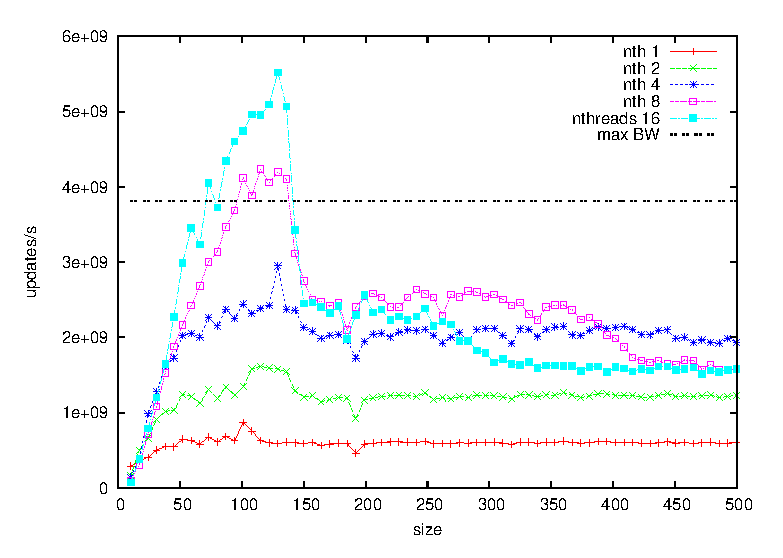
\includegraphics[scale=1.0]{./jacobi_idp_baseline.eps}
\caption{\label{fig:cpu} \small CPU three nested loops, double
  precision. Performace bounds to be added.}
\end{minipage}

\section{Many-cores architecture}

\begin{minipage}[t]{1.0\linewidth}
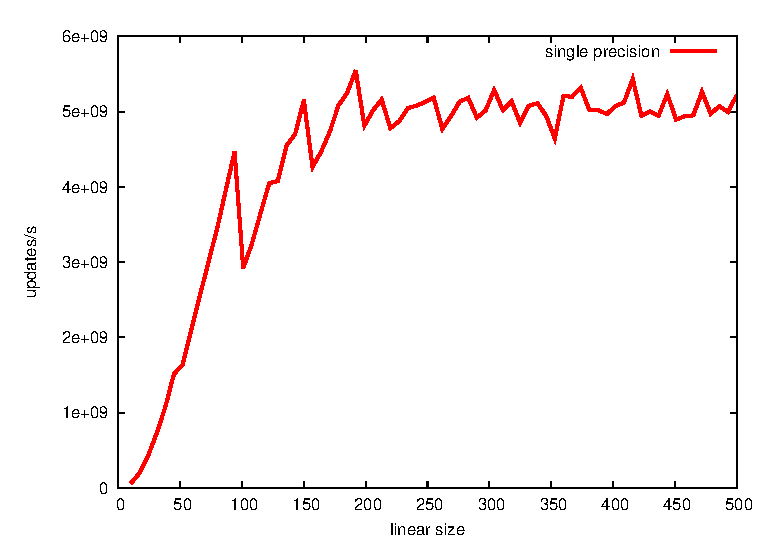
\includegraphics[scale=1.0]{./jacobi_gpu.eps}
\caption{\label{fig:gpu} \small GPU 2D block algorithm, single
  precision. Performace bounds to be added.}
\end{minipage}
\end{figure}
       
\begin{thebibliography}{1}
  \bibitem{Kamil} Shoaib Kamil, Parry Husbands, Leonid Oliker, John
  Shalf, Katherine Yelik, {\em Impact of Modern Memory Subsystems on
    Cache Optimisations for Stencil Computations}. In Proceedings of
  the 2005 workshop on Memory system performance (MSP '05). ACM, New
  York, NY, USA, 36-43 (2005).
\bibitem{Shah} Shah M. Faizur Rahman, Qing Yi, Apan Qasem, {\em
    Understanding Stencil Code Perfomance On MultiCore
    Architectures}. In Proceedings of the 8th ACM International
  Conference on Computing Frontiers (CF '11). ACM, New York, NY, USA (2011).
\bibitem{Treibig} Jan Treibig, Gerhard Wellein, Georg Hager, {\em
    Efficient multicore-aware parallelization srtategies for iterative
    stencil computations}, arXiv:1004.174v1 (2010).
  \bibitem{Holewinski} Justin Holewinski, Louis-Noël Pouchet,
  P. Sadayappan, {\em High-performance code generation for stencil
  computations on GPU architectures}. In Proceedings of the 26th ACM
  international conference on Supercomputing (ICS '12). ACM, New York,
  NY, USA, 311-320 (2012).
\end{thebibliography}


\end{document}


